\documentclass{article}
\usepackage[margin=1.25in]{geometry}
\usepackage{amsmath, amssymb}
\usepackage{graphicx}
\usepackage[T1]{fontenc}
\usepackage[utf8]{inputenc}
\usepackage{lmodern}
\usepackage[skip=10pt]{parskip}

\begin{document}

\begin{center}
	\textbf{\LARGE Sprawozdanie lista 1} \\
	{\large Marcin Wilk 261722} \\

\end{center}

\noindent \textbf{\large Zadanie 1}

\noindent \textbf{Opis problemu} \\
Sprawdzić jaki wpływ na dokładność wyników mają niewielkie zmiany danych \\
przy iloczynie skalarnym dwóch wektorów.

\noindent \textbf{Opis rozwiązania} \\
Porównać wyniki iloczynu skalarnego dwóch wektorów, w drugim przypadku usuwając
najmniej znaczące cyfry z dwóch składowych.

\noindent \textbf{Rezultat}

\noindent \textbf{Double}

\begin{center}
	\begin{tabular}{|l|l|l|}
		\hline
		\textbf{Faktyczny rezultat} & \textbf{Po kolei}       & \textbf{Po kolei (wstecz)} \\
		\hline
		$-1.00657107\cdot10^{-11}$  & $-0.004296342739891585$ & $-0.004296342998713953$    \\
		\hline
	\end{tabular}
\end{center}

\begin{center}
	\begin{tabular}{|c|c|}
		\hline
		\textbf{Od największych} & \textbf{Od najmniejszych} \\
		\hline
		$-0.004296342842280865$  & $-0.004296342842280865$   \\
		\hline
	\end{tabular}
\end{center}

\noindent \textbf{Float}

\begin{center}
	\begin{tabular}{|l|l|l|}
		\hline
		\textbf{Faktyczny rezultat} & \textbf{Po kolei} & \textbf{Po kolei (wstecz)} \\
		\hline
		$-1.00657107\cdot10^{-11}$  & $-0.4999443$      & $-0.4543457$               \\
		\hline
	\end{tabular}
\end{center}

\begin{center}
	\begin{tabular}{|c|c|}
		\hline
		\textbf{Od największych} & \textbf{Od najmniejszych} \\
		\hline
		$-0.5$                   & $-0.25$                   \\
		\hline
	\end{tabular}
\end{center}

\noindent \textbf{Wnioski} \\
Mała zmiana danych znacząco wpłynęła na błąd rozwiązania, powodując że wyniki
są praktycznie identyczne mimo różnych metod kalkulacji.

\noindent \textbf{\large Zadanie 2}

\noindent \textbf{Opis problemu} \\
Pokazać wykres $e^x*ln(1 + e^{-x})$ w dwóch programach rysujących wykresy.

\noindent \textbf{Opis rozwiązania} \\
Narysować wykres w dwóch program rysujących wykresy (w moim przypadku
matplotlib w pythonie oraz Plots w julii).

\pagebreak

\noindent \textbf{Rezultat}

\begin{center}
	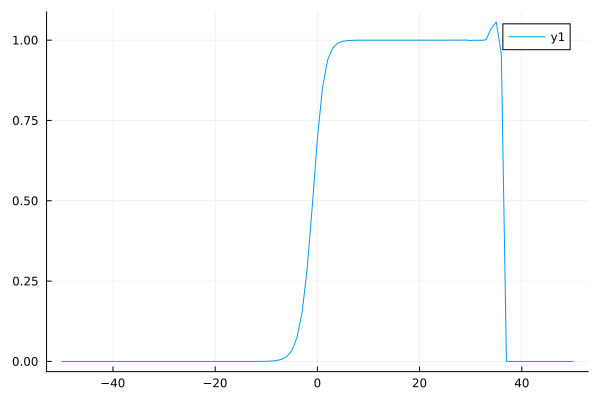
\includegraphics[scale=0.5]{plot.png}

	\textbf{Plots}
\end{center}

\begin{center}
	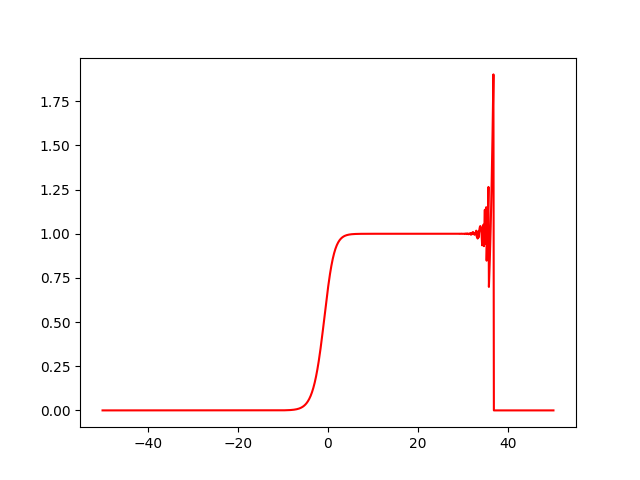
\includegraphics[scale=0.7]{zadanie2_python/plot.png}

	\textbf{matplotlib}
\end{center}

\noindent \textbf{Wnioski} \\
W pewnym momencie ta funkcja zaczyna dawać niepoprawne wyniki, a następnie
wpada do zera i utrzymuje się tam, mimo, że granica tej funkcji w nieskończności
to $1$. Dzieje się tak, ponieważ $e^{-a}$ w pewnym momencie jest już mniejsze od
epsilonu maszynowego i dodane do $1$ daje $1$ co przerzucone przez logarytm daje $0$.

\pagebreak

\noindent \textbf{\large Zadanie 3}

\end{document}
